%% -*- coding:utf-8 -*-
\chapter{Solutions to the exercises}


\section{Introduction and basic terms}


\eal
\ex \field{Karl}{VF} \field{isst}{LS}.
\ex \field{Der Mann}{VF} \field{liebt}{LS} \field{eine Frau}{MF}, \field{\field{den}{VF} \field{Peter}{MF} \field{kennt}{RS}}{NF}.
\ex \field{Der Mann}{VF} \field{liebt}{LS} \field{eine Frau, \field{die}{VF} \field{Peter}{MF} \field{kennt}{RS}}{MF}.
%\ex \field{Die Studenten}{VF} \field{behaupten}{LS}, \field{\field{nur wegen der Hitze}{MF} \field{einzuschlafen}{RS}}{MF}.
\ex \field{Die Studenten}{VF} \field{haben}{LS} \field{behauptet}{RS}, \field{\field{nur wegen der Hitze}{MF} \field{einzuschlafen}{RS}}{NF}.
\ex \field{\field{Dass}{LS} \field{Peter nicht}{MF} \field{kommt}{RS}}{VF}, \field{ärgert}{LS} \field{Klaus}{MF}.
\ex \field{\field{Einen Mann}{MF} \field{küssen}{RS}, \field{\field{der}{VF} \field{ihr nicht}{MF} \field{gefällt}{RS}}{NF}}{VF}, \field{würde}{LS} \field{sie nie}{MF}.
\zl
On (\mex{0}c): theoretically, this could also be a case of extraposition of the relative clause to
the postfield. Since \emph{eine Frau, die Peter kennt} is a constituent, however, it is assumed that
no reordering of the relative clause has taken place. Instead, we have a simpler structure with
\emph{eine Frau, die Peter kennt} as a complete NP in the middle field.


\section{Phrase structure grammars}



\begin{enumerate}
\item For any grammar, it is possible to assume additional symbols and rules that create unnecessary structure or are simply
never used because there are no words or phrases that could be used on the right"=hand side of the rule. If we were to add
the following rule to our grammar, for example, we would have a more complex grammar that can still analyze the same fragment
of the language.
\ea
Tralala $\to$ Trulla Trololo
\z
% \item Stellen Sie Überlegungen dazu an, wie man ermitteln kann, welche der unendlich vielen Grammatiken
%       die beste ist bzw.\ welche der Grammatiken die besten sind.
\item In general, it is assumed that the grammar with the fewest rules is the best one. Therefore, we can reject grammars that
contain unnecessary rules such as (\mex{0}).

One should bear in mind what the aim of a theory of grammar is. If our goal is to describe the human
language capacity, then a grammar with more rules could be better than other grammars with less
rules. This is because psycholinguistic research has shown that highly"=frequent units are simply
stored in our brains and not built up from their individual parts each time, although we would of
course be able to do this.\todostefan{Quelle und Beispiel}



\item The problem here is the fact that it is possible to derive a completely empty noun phrase
 (see Figure~\vref{Abbildung-leere-NP}). 
\begin{figure}
\centering
\begin{forest}
sm edges
[NP
  [Det [\trace]]
  [\nbar
    [N [\trace]]]]
\end{forest}
\caption{\label{Abbildung-leere-NP}Noun phrases without a visible determiner and noun}
\end{figure}%
This noun phrase could be inserted in all positions where an otherwise filled NP would have to stay. Then, we would
be able to analyze sequences of words such as (\mex{1}), where the subject of \emph{schläft} `sleeps' is realized
by an empty NP:
\ea[*]{
\gll Ich glaube, dass schläft.\\
     I believe that sleeps\\
}
\z
This problem can be solved using a feature that determines whether the left periphery of the \nbar is empty.
Visible Ns and \nbar with at least an adjective would have the value `--' and all others `+'. Empty determiners
could then only be combined with \nbar{}s that have the value `--'. See \citew{Netter94}.

\item %Überlegen Sie, warum es nicht sinnvoll ist, \emph{Bücher} als NP ins Lexikon zu schreiben.

If \emph{Bücher} `books' were an NP in the lexicon, then adjectives such as \emph{interessant} `interesting' would have to modify
NPs in order for phrases such as (\mex{1}) to be analyzed.
\ea
\gll interessante Bücher\\
     interesting books\\
\z
If adjectives are combined with NPs, however, it still has to be explained why (\mex{1}) is ungrammatical.
\ea[*]{
\gll interessante die Bücher\\
     interesting the books\\
}
\z

For a detailed discussions of this topic, see \citew[Section~6.6.2]{MuellerLehrbuch1}.\nocite{MuellerLehrbuch1}

\item %% Überlegen Sie, warum es auch nicht sinnvoll ist, die folgende Regel für Nomina wie \emph{Bücher} anzunehmen:
%% \ea
%% NP $\to$ Modifikator* Bücher Modifkator*
%% \z

This kind of rule cannot analyze noun phrases such as those in (\mex{1}):
\eal
\ex 
\gll interessante [Aufsätze und Bücher]\\
     interesting \spacebr{}essays and books\\
\ex 
\gll interessante [Aufsätze und Bücher aus Stuttgart]\\
     interesting \spacebr{}essays and books from Stuttgart\\
\zl
Since adjectives can only be combined directly with nouns, these phrases cannot be analyzed. 
 \emph{Bücher} `books' or \emph{Bücher aus Stuttgart} `books from Stuttgart' would be complete NPs.
 Since it is assumed that coordinated elements always have the same syntactic category, then \emph{Aufsätze} `essays'
 would have to be an NP. \emph{Aufsätze und Bücher} and \emph{Aufsätze und Bücher aus
  Stuttgart} would then also be NPs and it remains unexplained how an adjective can be combined with this NP.
Because of (\mex{-1}), we must rule out analyses that assume that full NPs combine with adjectives.

See Chapter~\ref{chap-empty} for a general discussion of empty elements.

\item 
% NP $\to$ the Adj
If a specific determiner or just any determiner were to be combined with an adjective to form a
complete NP, there would be no room for the integration of postnominal modifiers like modifying
genitives, PPs and relative clauses. For PPs and relative clauses, analyses have been suggested in
which these postnominal modifiers attach to complete NPs \citep{Kiss2005a}, but modifying genitives usually attach to
smaller units. But even if one admits postnominal modifiers to attach to complete NPs, one cannot
account for the iteration of adjectives and for arguments that depend on the elided noun.
 
So, the simplest way to cope with the German data is the assumption of an empty noun. Alternatively
one could assume that an adjective is directly projected to an \nbar. This \nbar then can be
modified by further adjectives or postnominal modifiers. The \nbar is combined with a determiner to
form a full NP. For phrases that involve elided relational nouns, one would have to assume the projection of an argument like \emph{vom Gleimtunnel} `of the
Gleimtunnel' to  \nbar. The \nbar could be further modified or combined with a determiner directly.

%\item Überlegen Sie sich, warum die \xbart mit deutschen Adjektivphrasen nicht ohne Zusatzannahmen
%klarkommt.
\item Adjective phrases such as those in (\mex{1}) cannot be analyzed since the degree modifier
occurs between the complement and the adjective:
\ea
\gll der auf seinen Sohn sehr stolze Vater\\
	 the on his son very proud father\\
\glt `the father very proud of his son'
\z
One would either have to allow for specifiers to be combined with their heads before complements or allow crossing lines in trees. Another assumption
could be that German is like English, however then adjectival complements would have to be obligatorily reordered before their specifier. For
a description of this kind of reordering, see Chapter~\ref{Kapitel-GB}. See Section~\ref{sec-Diskussion-X-Bar} for a discussion of \xbar"=Theory.

\item Write a phrase structure grammar that can analyze the sentences in (\mex{1}), but does not allow the strings of words in (\mex{2}).
      \eal
      \ex[]{
      \gll Der Mann hilft der Frau.\\
           the.\nom{} man helps the.\dat{} woman\\
      \glt `The man helps the woman.'
      }
      \ex[]{
      \gll Er gibt ihr das Buch.\\
           he.\nom{} gives her.\dat{} the.\acc{} book\\
      \glt `He gives her the book.'
      }
      \ex[]{
      \gll Er wartet auf ein Wunder.\\
	   he.\nom{} waits on a miracle.\acc{}\\
      \glt `He is waiting for a miracle.'
      }
%       \ex[]{
%       Er wartet neben dem Bushäuschen auf ein Wunder.
%       }
      \zl
      \eal
      \ex[*]{
        \gll Der Mann hilft er.\\
             the.\nom{} man helps he.\nom{}\\
      }
      \ex[*]{
       \gll Er gibt ihr den Buch.\\
	    he.\nom{} gives her.\dat the.\acc{} book\\
      }
      \zl

In order to rule out the last two sentences, the grammar has to contain information about case. The following grammar will do the job:
\eal
\ex s $\to$ np(nom) v(nom\_dat), np(dat)
\ex s $\to$ np(nom), v(nom\_dat\_acc), np(dat), np(acc)
\ex s $\to$ np(nom), v(nom\_pp\_auf), pp(auf,acc)
\ex pp(Pform,Case) $\to$ p(Pform,Case), np(Case)
\ex np(Case) $\to$ d(Case), n(Case)
\ex v(nom\_dat) $\to$ hilft
\ex v(nom\_dat\_acc) $\to$ gibt
\ex v(nom\_pp\_auf) $\to$ wartet
\ex np(nom) $\to$ er
\ex np(dat) $\to$ ihr
\ex d(nom) $\to$ der
\ex d(dat) $\to$ der
\ex d(acc) $\to$ das
\ex d(acc) $\to$ ein
\ex n(nom) $\to$ Mann
\ex n(dat) $\to$ Frau
\ex n(acc) $\to$ Buch
\ex n(acc) $\to$ Wunder
\ex p(auf,acc) $\to$ auf
\zl

% \item Installieren Sie ein Prolog"=System (\zb SWI"=Prolog\footnote{
% \url{http://www.swi-prolog.org/}
% }) und probieren Sie Ihre Grammatik aus.
\end{enumerate}



\section{Transformational Grammar -- Government \& Binding}


% \ex dass die Frau den Mann liebt
% \ex dass der Mann geliebt wird
% \ex Der Mann wird geliebt.
% \ex dass der Mann der Frau hilft
% \ex Der Mann hilft der Frau.

\begin{figure}[H]
\centering
\scalebox{.9}{%
\begin{forest}
sm edges
[CP
[C$'$
	[C$^0$[dass;that]]
	[IP
		[NP [die Frau;the woman,roof]]
		[I$'$
			[VP
				[V$'$
					[NP[den Mann;the man, roof]]
					[V$^0$[\trace$_j$]]]]
			[I$^0$[lieb-$_j$ -t;love- -s]]]]]]
\end{forest}
}
%\end{figure}%
\hfill
% dass der Mann geliebt wird
%\begin{figure}[H]
\scalebox{.9}{
\begin{forest}
sm edges
[CP
[C$'$
	[C$^0$[dass;that]]
        [IP
        [NP, [der Mann$_i$;the man ,roof]]
        [I$'$
	   [VP
		[V$'$
	           [NP,   [\_$_i$]]
		   [V$^0$,[geliebt \trace$_j$;loved, roof]]]]
	   [I$^0$ ,name=Infl [wir-$_j$ -d;is]]]]]]
\end{forest}
}
\end{figure}%


% der Mann wird geliebt
\begin{figure}[H]
\scalebox{.9}{%
\begin{forest}
sm edges
[CP
   [NP, [der Mann$_i$;the man ,roof]]
   [C$'$
	[C$^0$[ (wir-$_j$ -d)$_k$;is]]
        [IP
        [NP, [\trace$_i$]]
        [I$'$
	   [VP
		[V$'$
	           [NP,   [\_$_i$]]
		   [V$^0$,[geliebt \trace$_j$;loved, roof]]]]
	   [I$^0$ ,name=Infl [\trace$_k$]]]]]]
\end{forest}
}
%\end{figure}%
\hfill
% \ex dass der Mann der Frau hilft
%\begin{figure}[H]
%\centering
\scalebox{.9}{%
\begin{forest}
sm edges
[CP
[C$'$
	[C$^0$[dass;that]]
	[IP
		[NP [der Mann;the man, roof]]
		[I$'$
			[VP
				[V$'$
					[NP[der Frau;the woman, roof]]
					[V$^0$[\trace$_j$]]]]
			[I$^0$[hilf-$_j$ -t;help- -s]]]]]]
\end{forest}
}
\end{figure}%

% \ex Der Mann hilft der Frau.
\begin{figure}[H]
\centering
\begin{forest}
sm edges
[CP
[NP [der Mann$_i$;the man, roof]]
[C$'$
	[C$^0$ [(hilf-$_j$ -t)$_k$;help- -s]]
	[IP
		[NP [\trace$_i$]]
		[I$'$
			[VP
				[V$'$
					[NP [der Frau;the woman, roof]]
					[V$^0$[\trace$_j$]]]]
			[I$^0$ [\trace$_k$]]]]]]
\end{forest}
\end{figure}%

%\clearpage

\section{Generalized Phrase Structure Grammar}

In order to analyze the sentences in (\mex{1}), one requires a rule for transitive verbs and a metarule for the extraction of an element.
Furthermore, rules for the combination of elements in the noun phrase are required.
\eal
\label{Aufgabe-GPSG-Grammatik}
\ex 
\gll {}[dass] der Mann ihn liest\\
	 {}\spacebr{}that the man it reads\\
\glt `that the man reads it'
\ex 
\gll {}[dass] ihn der Mann liest\\
	{}\spacebr{}that it the man reads\\
\glt `that the man reads it'
%\ex {}[dass] er gelesen wurde
\ex\label{Aufgabe-GPSG-Grammatik-extraction}
\gll Der Mann liest ihn.\\
     the man reads it\\
\glt `The man reads it.'
\zl

\noindent
It is possible to analyze the sentences in (\mex{0}a,b) using the rules in (\mex{1}) and the lexical entries in (\mex{2}).
\eal
\ex V3 $\to$ H[6], N2[\textsc{case} nom], N2[\textsc{case} acc] 
\ex N2 $\to$ Det[\textsc{case} CAS], H1[\textsc{case} CAS]
\ex N1 $\to$ H[27]
\zl

\eal
\ex Det[\textsc{case} nom] $\to$ der
\ex N[27] $\to$ Mann
\ex V[6, $+$\textsc{fin}] $\to$ liest
\ex N2[\textsc{case} acc] $\to$ ihn
\zl

\noindent
The rules (\mex{-1}b,c) correspond to \xbar-rules that we encountered in Section~\ref{sec-psg-np}. They only differ from these rules
in that the part of speech of the head is not given on the right"=hand side of the rule. The part of speech is determined by
the Head Feature Convention. The part of speech of the head is identical to that on the left"=hand
side of the rule, that is, it must be N in (\mex{-1}b,c). It also follows from the Head Feature Convention that the
whole NP has the same case as the head and therefore does not have to be mentioned additionally in
the rule above. 27 is the \subcatv. This number is arbitrary. 

In order for the verb to appear in the correction position, we need linearization rules:
\ea
\begin{tabular}[t]{@{}l@{~$<$~}l@{}}
V[+\textsc{mc}]  & X\\
X       & V[$-$\textsc{mc}]\\
\end{tabular}
\z
The fact that the determiner precedes the noun is ensured by the following LP"=rule:
\ea
{}Det $<$ X
\z
\pagebreak
The Extraction Metarule in (\mex{1}) is required in order to analyze (\ref{Aufgabe-GPSG-Grammatik-extraction}):
\ea
V3  $\to$ W, X $\mapsto$\\
V3/X  $\to$ W
\z
Among others, this metarule licenses the rule in (\mex{1}) for (\mex{-4}a):
\ea
V3/N2[\textsc{case} nom]  $\to$ H[6],  N2[\textsc{case} acc] 
\z

\noindent
The rule in (\mex{1}) is used to bind off long"=distance dependencies.
\ea
V3[+\textsc{fin}] $\to$ X[+\textsc{top}], V3[+\textsc{mc}]/X
\z
The following linearization rule ensures that the $+$\textsc{top}-constituent precedes the sentence in which it is missing:
\ea
{}[+\textsc{top}] $<$ X
\z

\noindent
Figure~\vref{fig-der-mann-liest-ihn} shows the structure licensed by the grammar.
\begin{figure}
\centering
\begin{forest}
sm edges
[{V3[+\textsc{fin}, $+$\textsc{mc}]}
   [{N2[nom, $+$\textsc{top}]} [der Mann;the man, roof]]
   [{V3[+\textsc{mc}]/N2[nom]}
     [{V[6, $+$\textsc{mc}]} [liest;reads]]
     [{N2[acc]} [ihn;him]]]]
\end{forest}
\caption{\label{fig-der-mann-liest-ihn}Analysis of \emph{Der Mann liest ihn.} `The man reads it.'}
\end{figure}%
In sum, one can say that the grammar that licenses the sentences in (\ref{Aufgabe-GPSG-Grammatik}) should have (at least) the following
parts:

\begin{enumerate}
\item ID rules:
\eal
\ex V3 $\to$ H[6], N2[\textsc{case} nom], N2[\textsc{case} acc] 
\ex N2 $\to$ Det[\textsc{case} CAS], H1[\textsc{case} CAS]
\ex N1 $\to$ H[27]
\zl
\item LP rules:
\ea
\begin{tabular}[t]{@{}l@{~$<$~}l@{}}
V[+\textsc{mc}]  & X\\
X       & V[$-$\textsc{mc}]\\
Det     & X\\
{}[+\textsc{top}] & X\\
\end{tabular}
\z
\pagebreak
\item Metarules:
\ea
V3  $\to$ W, X $\mapsto$\\
V3/X  $\to$ W
\z


\item Lexical entries
\eal
\ex Det[\textsc{case} nom] $\to$ der
\ex N[27] $\to$ Mann
\ex V[6, $+$\textsc{fin}] $\to$ liest
\ex N2[\textsc{case} acc] $\to$ ihn
\zl

\end{enumerate}

\section{Feature descriptions}

\begin{enumerate}
%% \item Geben Sie eine Typhierarchie für Wortarten (\type{det}, \type{comp}, \type{noun}, \type{verb},
%%       \type{adj}, \type{prep}) an. Überlegen Sie, wie man die Typhierarchie so
%%       formulieren kann, dass sie es ermöglicht, die Generalisierungen auszudrücken, die man auch mit
%%       der Merkmalszerlegung in Tabelle~\ref{Tabelle-Merkmalszerlegung-Wortarten} auf
%%       Seite~\pageref{Tabelle-Merkmalszerlegung-Wortarten} ausdrücken kann.

\item For\todostefan{Musikinstrumente fehlt noch}
 the class [+V], the type \type{verbal} is assumed with the subtypes \type{adjective} and
  \type{verb}. For the class [$-$V] there is the type \type{non-verbal} and its subtypes \type{noun} and
  \type{preposition}. This is analogous for the N values. The corresponding hierarchy is given in the following
  figure:
\begin{figure}[H]
\centering
\begin{forest}
typehierarchy
[p-o-s, for descendants={l sep+=5mm}
  [nominal,     name=nominal,        [adjective,   name=adjective]]
  [non-nominal, name=nonnominal,     [verb,        name=verb]]
  [verbal,      name=verbal,         [noun,        name=noun, no edge]]
  [non-verbal,  name=nonverbal,      [preposition, name=preposition]] ]
\draw (nominal.south)    --(noun.north)
      (nonnominal.south) --(preposition.north)
      (verbal.south)     --(adjective.north)
      (verbal.south)     --(verb.north)
      (nonverbal.south)  --(noun.north);
\end{forest}
\end{figure}%

\item Lists\is{list} can be described using recursive structures that consist of both a list beginning and a rest. The rest can either
be a non"=empty list (\type{ne\_list}) or the empty list (\type{e\_list}). The list \relliste{ \type{a}, \type{b}, \type{c} } can be represented as follows:
\ea
\ms[ne\_list]{
first & a\\
rest  & \ms[ne\_list]{
        first & b\\
        rest  & \ms[ne\_list]{
                first & c\\
                rest & e\_list\\
                }\\
        }\\
}
\z
\item If we extend the data structure in (\mex{0}) by two additional features, it is possible to do without
  \emph{append}. The keyword is  \emph{difference list}\is{list!difference}. A difference list consists of a list
  and a pointer to the end of the list.
\ea
\ms[diff-list]{
list & \ms[ne\_list]{
       first & a\\
       rest  & \ms[ne\_list]{
               first & b\\
               rest  & \ibox{1} list\\
               }\\
       } \\
last & \ibox{1}\\
}
\z

Unlike the list representation in (\mex{-1}), the \textsc{rest} value of the end of the list is not \type{e\_list}, but rather
simply \type{list}. It is then possible to extend a list by adding another list to the point where it ends. The concatenation of 
(\mex{0}) and (\mex{1}a) is (\mex{1}b).
\eal
\ex 
\ms[diff-list]{
list & \ms[ne\_list]{
       first & c\\
       rest  & \ibox{2} list\\
       } \\
last & \ibox{2}\\
}
\ex
\ms[diff-list]{
list & \ms[ne\_list]{
       first & a\\
       rest  & \ms[ne\_list]{
               first & b\\
               rest  & \ms[ne\_list]{
                       first & c\\
                       rest  & \ibox{2} list\\
                       }\\
               }\\
       } \\
last & \ibox{2}\\
}
\zl
In order to combine the lists, the \textsc{list} value of the second list has to be identified with the {\sc
  last} value of the first list. The \textsc{last} value of the resulting list then corresponds to the
  \textsc{last} value of the second list (\ibox{2} in the example.)

Information about the encoding of difference lists can be found by searching for the keywords  \emph{list}, \emph{append}, and
\emph{feature structure}. In the search results, one can find pages on developing grammars that explain
difference lists.
\end{enumerate}



\section{Lexical Functional Grammar}

\begin{enumerate}
\item \emph{kannte} `knew' is a transitive verb:
\ea
\catlexentry{kannte}{V}{(\up\ \pred) = {\small `KENNEN\arglist{\subj, \obj}'}\\*
                        (\up\ \subj{} {\small AGR CAS} = NOM)\\*
                        (\up\ \obj{} {\small AGR CAS} = ACC)\\*
                        (\up\ \lfgtense) = \small PAST}
\z

\item In the sentence (\mex{1}), the object of \emph{verschlingen} `devour' is in the prefield.
\ea
\gll Den Apfel verschlingt David.\\
	 the.\acc{} apple devours David.\nom\\
\glt `David is devouring the apple.'
\z
The analysis is a combination of the analysis in Figure~\vref{Abb-Verbstellung-LFG} and the analysis of long"=distance
dependencies that was presented in Section~\ref{Abschnitt-NLA-LFG}. The object is not realized inside the VP, but rather
in the prefield.

The necessary c"=structure rules are given in (\mex{1}):
\eal
\ex 
\phraserule{VP}{
\rulenode{NP\\* (\up \subj|\obj) = \down}
\rulenode{VP\\* \up = \down}}
\ex
\phraserule{VP}{
\rulenode{(V)\\* \up = \down}}
\ex
\phraserule{C$'$}{
\rulenode{C\\* \up = \down}
\rulenode{VP\\* \up = \down}}
\ex 
% \phraserule{CP}{
% \rulenode{XP\\* (\up \textsc{df}) = \down\\* (\up \textsc{df}) = (\up \textsc{comp obj}) }
% \rulenode{C$'$\\* \up = \down}}
%
\begin{tabular}[t]{@{}ccc@{~=~}lc@{}}
CP & $\rightarrow$ & \multicolumn{2}{l}{\hspaceThis{(\up \textsc{df})}XP} & C$'$ \\
 & &  (\up \textsc{df}) & \down & \up=\down \\
 & &  (\up \textsc{df}) & (\up \textsc{comp* gf})\\
\end{tabular}
\zl

\noindent
These rules allow two f"=structures for the example in question: one in which the NP \emph{den
  Apfel} `the apple' is the topic and another in which this NP is the focus. Figure~\ref{Abbildung-V2-LFG} 
shows the analysis with a topicalized constituent in the prefield.\todostefan{Dreieck für den Apfel}

\begin{figure}
\centerline{%
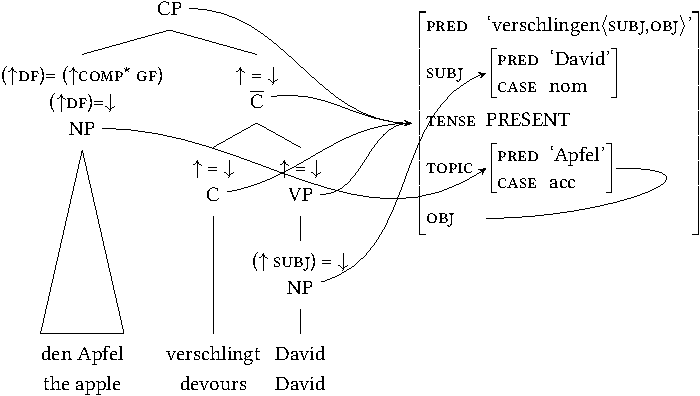
\includegraphics{Figures/den-apfel-verschlingt-david-lfg-lsp-crop}
}
\caption{\label{Abbildung-V2-LFG}Analysis of verb second}
\end{figure}%
\end{enumerate}

\pagebreak
\section{Categorial Grammar}

\largerpage
\begin{enumerate}
\item The analysis of \emph{The children in the room laugh loudly.} is given in Figure~\ref{Abbildung-CG-Kinder-lachen-laut}.
\begin{figure}[H]
\centerline{%
\deriv{7}{
the   & children  & in  & the      & room                 & laugh & loudly\\
\hr   & \hr       & \hr & \hr      & \hr                    & \hr     & \hr \\
%
%
np/n  & n       & (n\bs n)/np & np/n & n                & s\bs np  & (s\bs np)\bs (s\bs np)\\
      &         &             & \multicolumn{2}{c}{\forwardapp} & \multicolumn{2}{c@{}}{\backwardapp}\\
      &         &             & np\\
      &         & \multicolumn{3}{c}{\forwardapp}  & \multicolumn{2}{c@{}}{s\bs np}\\
%
%
      &         & \multicolumn{3}{c}{n\bs n} \\  
      & \multicolumn{4}{c}{\backwardapp}\\
      & \multicolumn{4}{c}{{{n}}}\\
%
\multicolumn{5}{@{}c}{\forwardapp}\\
\multicolumn{5}{@{}c}{{np}}\\
%
\multicolumn{7}{@{}c@{}}{\backwardapp}\\
\multicolumn{7}{@{}c@{}}{{s}}\\
}}
\caption{\label{Abbildung-CG-Kinder-lachen-laut}Categorial Grammar analysis of \emph{The children in
    the room laugh loudly.}}
\end{figure}%

\item The analysis of \emph{the picture of Mary} is given in
  Figure~\vref{Abbildung-CG-das-Bild-von-Maria}. n/pp corresponds to \nnull, n corresponds to \nbar
  and np corresponds to NP.
\begin{figure}[H]
\centerline{%
\deriv{4}{
the & picture & of & Mary\\
\hr   & \hr     & \hr        & \hr\\
np/n  & n/pp    & pp/np      & np\\
%
      &         & \multicolumn{2}{c@{}}{\forwardapp}\\
      &         & \multicolumn{2}{c@{}}{pp}\\
%
      & \multicolumn{3}{c@{}}{\forwardapp}\\
      & \multicolumn{3}{c@{}}{n}\\
%
\multicolumn{4}{@{}c@{}}{\forwardapp}\\
\multicolumn{4}{@{}c@{}}{np}\\
}}
\caption{Categorial Grammar analysis of \emph{the picture of Mary}\label{Abbildung-CG-das-Bild-von-Maria}}
\end{figure}%
\end{enumerate}

\section{Head-Driven Phrase Structure Grammar}

\largerpage
\begin{enumerate}
\item The solution is:\\[1mm]
%\vpageref{avm-max-lacht}.
%\begin{figure}
\oneline{%
\onems[head-argument-phrase~]{
      phon  \phonliste{ Max lacht }\\
      synsem$|$loc \ms{ cat \ms{ head & \ibox{1}\\
                                 subcat & \ibox{2} \eliste \\
                               }\\
                        cont \ms{ ind & \ibox{3}  \\
                                       rels & \relliste{ \ibox{4}, \ibox{5} } \\
                                     }\\
                      }\\
      head-dtr \onems[word]{ phon \phonliste{ lacht }\\
                             synsem$|$loc  \ms{ cat & \ms{ head   & \ibox{1} \ms[verb]{ initial & $-$\\
                                                                                        vform   & fin \\
                                                                                   }\\
                                                            subcat & \ibox{2}  $\oplus$ \sliste{ \ibox{6} }  \\
                                                        }\\
                                                 cont & \ms{ ind & \ibox{3} event \\
                                                                  rels & \liste{ \ibox{4} \ms[lachen]{ event & \ibox{3} \\
                                                                                                       agens & \ibox{7} \\ }} \\
                                                                }
                                               }\\
                       } \\
      non-head-dtrs \liste{ \onems[word]{ 
                                        phon \phonliste{ Max }\\
                                        synsem \ibox{6} \onems{ loc \ms{ cat & \ms{ head   & \ms[noun]{ cas & nom\\
                                                                                                      } \\
                                                                                    subcat &  \eliste \\
                                                                                }\\
                                                                         cont & \ms{ ind & \ibox{7} \ms{ per & 3 \\
                                                                                                              num & sg \\
                                                                                                              gen & mas \\
                                                                                                            } \\
                                                                                          rels & \liste{
                                                                                                  \ibox{5} \ms[named]{ name & max    \\
                                                                                                                       inst & \ibox{7} \\ }} \\
                                                                                         } \\
                                                                        }\\
                                                              }\\
                                   } 
                           } \\
}}
\label{avm-max-lacht}
%\end{figure}%
\item An analysis of the difference in (\mex{1}) has to capture the fact that the case of the adjective has to agree with that of the noun. In (\mex{1}a),
the genitive form of \emph{interessant} `interesting' is used, whereas (\mex{1}b) contains a form that is incompatible with the genitive singular.
\eal
\ex[]{
\gll eines interessanten Mannes\\ 
     one.\gen{} interesting.\gen{} man.\gen{}\\
}
\ex[*]{ 
\gll eines interessanter Mannes\\
     one.\gen{} interesting.\nom{} man.\gen{}\\
}
\zl
(\mex{1}) shows the \catv of \emph{interessanten}.

\eas
\catv of \emph{interessanten} `interesting' with case information:\\
\ms{ head & \ms[adj]{ %prd & $-$ \\
                      mod  & {\upshape \nbar[\textsc{case} \ibox{1}]}\\
                      case & \ibox{1} gen\\
                    } \\
              subcat & \liste{} \\
}
\zs
The structure sharing of the case value of the adjective with the case value of the \nbar under \textsc{mod}
identifies the case values of the noun and the adjective. \emph{interessanten} can therefore be combined with 
\emph{Mannes}, but not with \emph{Mann}. Similarly, \emph{interessanter}
can only be combined with the nominative \emph{Mann}, but not with the genitive \emph{Mannes}. 

For a refinement of the analysis of agreement inside the noun phrase, see \citew[Abschnitt~13.2]{MuellerLehrbuch1}.
\end{enumerate}


\section{Construction Grammar}

Idioms can be found by reading the newspaper carefully. The less exciting method is to look them up a dictionary of
idioms such as the Free Dictionary of Idioms and Phrases\footnote{
\url{http://idioms.thefreedictionary.com/}, 04.03.2015.
}.


\section{Dependency Grammar}

\begin{figure}[H]
\centering
\scalebox{.9}{%
\begin{forest}
dg edges
[V
  [N [ich;I]]
  [habe;have]
  [N,name=n
    [Det,tier=det [einen;a]]
    [Mann;man]]
  [V [getroffen;met]]
  [Rel,no edge, tier=det,name=rel [\trace]
      [V
        [N [der;who]]
        [N [Adj, dg adjunct [blonde;blond]]
           [Haare;hair]]
        [hat;has]]]]
\draw (n.south)--(rel.north)-- +(0,6pt);
\end{forest}
}
\end{figure}%

\begin{figure}[H]
\centering
\scalebox{.9}{%
\begin{forest}
dg edges
[V
  [Subjunction
    [dass;that]
    [V, l sep+=15pt
      [N [er;he]]
      [Adv, dg adjunct [morgen;tomorrow]]
      [V [kommen;come]]
      [wird;will]]]
  [freut;pleases]
  [N [uns;us]]]
\end{forest}
}
\end{figure}%

\begin{figure}[H]
\centering
\scalebox{.9}{
\begin{forest}
dg edges
[V
  [V [N,name=n
       [Det,tier=det [einen;a]]
       [Mann;man]]
    [getroffen;met]]
  [Rel,no edge, tier=det,name=rel [\trace]
      [V
        [N [der;who]]
        [N [Adj, dg adjunct [blonde;blond]]
           [Haare;hair]]
        [hat;has]]]
  [habe;have]
  [N [ich;I]]
  [Adv [noch;yet]]
  [Adv [nie;never]]]
\draw (n.south)--(rel.north)-- +(0,6pt);
\end{forest}
}
\end{figure}%






\section{Tree Adjoining Grammar}

%\addlines[2]
The elementary trees in Figure~\vref{TAG-Elementarbaeume-dem-Koenig-treue} are needed for the analysis of (\mex{1}).
\ea
\gll der        dem        König treue Diener\\
     the.\nom{} the.\dat{} king  loyal servant\\
\glt `the servant loyal to the king'
\z

\begin{figure}
\hfill
\scalebox{.9}{
\begin{forest}
tag
[Det [der;the]]
\end{forest}
}
\hfill
\scalebox{.9}{
\begin{forest}
tag
[Det [dem;the]]
\end{forest}
}
\hfill
\scalebox{.9}{
\begin{forest}
tag
[NP
  [Det$\downarrow$]
  [N$'$
    [N [König;king]]]]
\end{forest}
}
%
\hfill
%
\scalebox{.9}{
\begin{forest}
tag
[N$'$
  [AP
    [A$'$
      [NP$\downarrow$]
      [A [treue;loyal]]]]
  [N$'$*]]
\end{forest}
}
%
\hfill
%
\scalebox{.9}{
\begin{forest}
tag
[NP
  [Det$\downarrow$]
  [N$'$
    [N [Diener;servant]]]]
\end{forest}
}
\hfill\mbox{}
\caption{\label{TAG-Elementarbaeume-dem-Koenig-treue}Elementary trees for \emph{der dem König treue Diener}}
\end{figure}%

\noindent
By substituting the tree for \emph{dem} `the' in the substitution node of \emph{König} `king', one then arrives at a full NP.
This can then be inserted into the substitution node of \emph{treue} `loyal'. Similarly, the tree
for \emph{der} `the' can be combined with the one for \emph{Diener}. One then has both of the trees in Figure~\vref{TAG-substituiert}.

\begin{figure}
\hfill
\scalebox{.9}{
\begin{forest}
tag
[N$'$
  [AP
    [A$'$
      [NP
        [Det [dem;the]]
        [N$'$
          [N [König;king]]]]
      [A [treue;loyal]]]]
  [N$'$*]]
\end{forest}
}
%
\hfill
\scalebox{.9}{
\begin{forest}
tag
  [NP
     [Det [der;the]]
     [N$'$
        [N [Diener;servant]]]]
\end{forest}
}
\hfill\mbox{}
\caption{\label{TAG-substituiert}Trees for \emph{der dem König treue} and \emph{der Diener} after substitution}
\end{figure}%
The adjective tree can then be adjoined to the N$'$"=node of \emph{der Diener}, which yields the structure in Figure~\vref{TAG-Baeume-nach-Adjunktion}.
\begin{figure}
\centering
%\scalebox{.9}{
\begin{forest}
tag
  [NP
     [Det [der;the]]
     [N$'$
       [AP
         [A$'$
           [NP
             [Det [dem;the]]
             [N$'$
               [N [König;king]]]]
           [A [treue;loyal]]]]
       [N$'$
         [N [Diener;servant]]]]]
\end{forest}
%}
\caption{\label{TAG-Baeume-nach-Adjunktion}Result of adjunction of the AP to the N$'$"=node}
\end{figure}%




%      <!-- Local IspellDict: en_US-w_accents -->
